\section{Tracking}

The drift chamber, with 112 layers of wires, provides high number of measurements which can be exploited for the track reconstruction.

One of the methods we are investigated is the Hough transform as described below.

\subsection{The Hough Transform}
Initially invented for bubble chamber photographs~\cite{HTWikipedia}, the Hough Transform is a feature extraction technique used in several fields such as image analysis, computer vision and digital image procession. It allows for the identification of lines as well as other shapes such as circles or ellipses.

\subsubsection{Principle}
The simplest case of Hough transform is detecting straight lines. In the parameter space, lines are represented as a point (b, m) with \cref{lineeq}.

\begin{equation}
	y = m \cdot x + b
	\label{lineeq}
\end{equation}

\begin{figure}[ht]

	\centering
	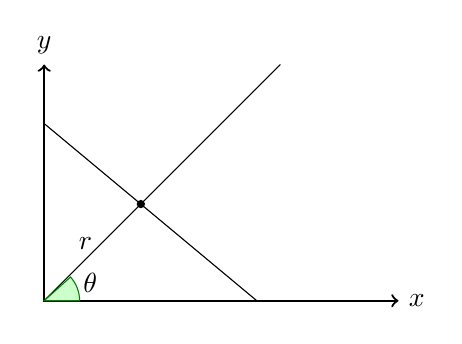
\begin{tikzpicture}[scale=1.5]
    % Draw axes
    \draw [<->,thick] (0,2) node (yaxis) [above] {$y$}
        |- (3,0) node (xaxis) [right] {$x$};
    % Draw two intersecting lines
    \draw (0,0) coordinate (a_1) -- (2, 2) coordinate (a_2);
    \draw (0,1.5) coordinate (b_1) -- (1.8,0) coordinate (b_2);

    \coordinate (c) at (intersection of a_1--a_2 and b_1--b_2);

		\filldraw[fill=green!20,draw=green!50!black] (0,0) -- (3mm,0mm) arc (0:42:3mm) -- cycle;
		\node[right] at (0.25, 0.15) {$\theta$};
		\node[above] at (0.35, 0.35) {$r$};
		% right angle
    \fill[black] (c) circle (1pt);


\end{tikzpicture}
\caption{A line is represented as a point (b, m) in the parameter space or (r, $\theta$) in the Hough space according to \cref{lineeq,line_hesse}.}
\label{fig_lineParamSpace}
\end{figure}

With the presentation (b, m) in the parameter space, vertical lines pose problems for the unbounded slope parameter \textit{m}. The Hesse normal form as described in \cref{line_hesse} can be used as a solution to get around vertical lines, where $r$ is the shortest distance from the origin to the line and $\theta$ is the angle between the $x$ axis and the line connecting the origin with the closest point as illustrated in \cref{fig_lineParamSpace}. The (r,~$\theta$) plane is referred to as the Hough Space.


\begin{equation}
	r = x \cdot \cos(\theta) + y \cdot \sin(\theta)
	\label{line_hesse}
\end{equation}

\cref{HTLine} shows the Hough transformation applied to every point on a line. In the Hough space, all the points on the line are represented by a local maximum since they all have the same (r,~$\theta$) value.
\begin{figure}[ht]
	\centering
	\begin{subfigure}[b]{0.45\textwidth}
        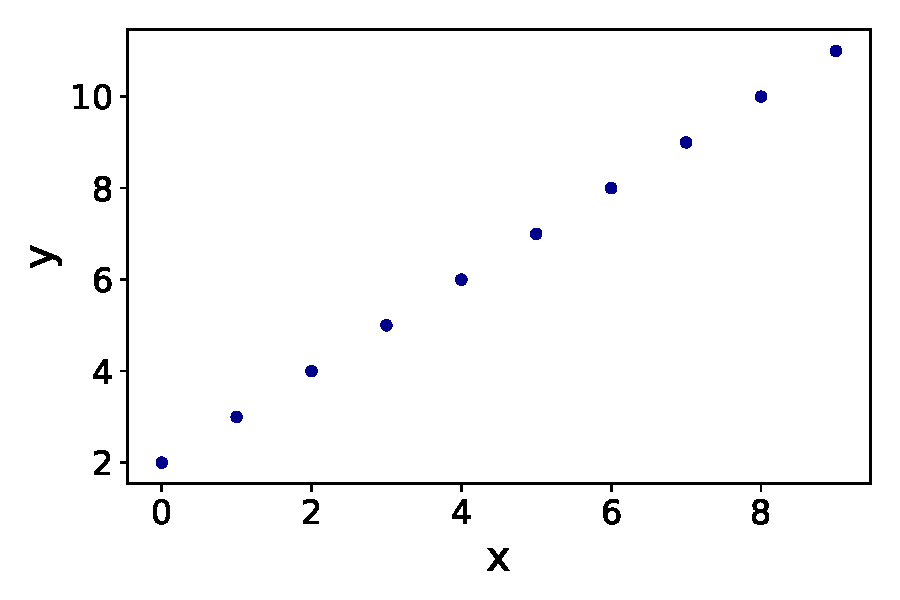
\includegraphics[width=\textwidth]{figures/line.pdf}
        \caption{Parameter space}
        % \label{pointsLine}
    \end{subfigure}
		~ %
		\begin{subfigure}[b]{0.45\textwidth}
					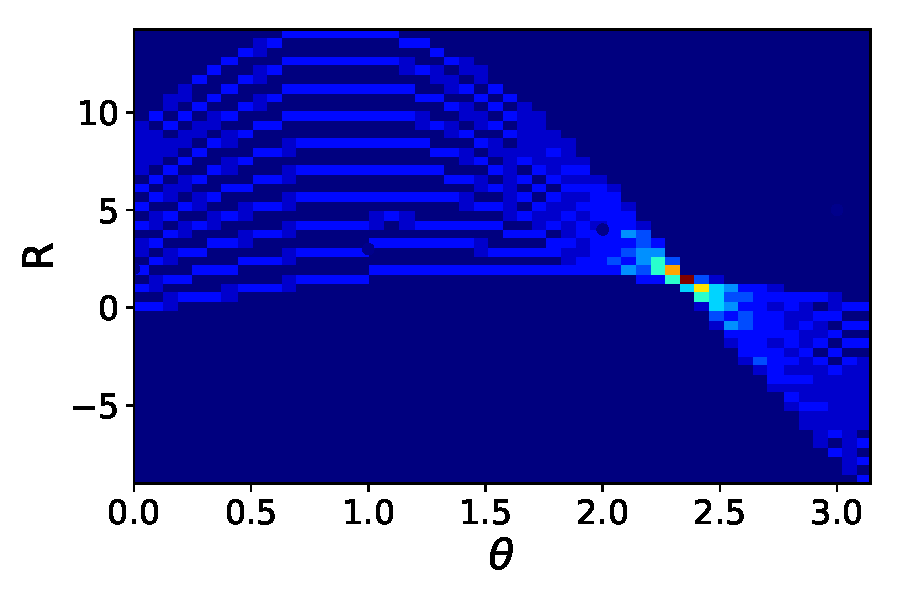
\includegraphics[width=\textwidth]{figures/line_hough.pdf}
					\caption{Hough space}
					% \label{pointsLine2}
			\end{subfigure}
	\label{HTLine}
	\caption{A line as represented in the parameter and the Hough space.}
\end{figure}

\subsubsection{Identification of circles}

The track of a charged particle in a magnetic field follows a helicoidal trajectory. In the xy-plane, the hits follow a circular trajectory as described with \cref{circleEq} where $(a, b)$ represent the center of the circle and $R$ the radius of the circle.

\begin{equation}
  {(x-a)}^2 + {(y-b)}^2 = R^2
	\label{circleEq}
\end{equation}

The Hough transformation gets better results when applied to lines. For this reason, first the conformal mapping~\cite{Hansroul:1988wa} is first applied to map circular hits into lines using \cref{conformalTrans}.

\begin{equation}
  u = {{x} \over {x^2+y^2}} , \,\,\,\, v = {{y} \over {x^2+y^2}}
	\label{conformalTrans}
\end{equation}

The conformal mapping maps a circle to a line if and only if the circle passes from the origin or following the condition as described in \cref{conformalTrans_condition} and the straight lines are described by \cref{equation_straightLine}.

\begin{equation}
  a^2 + b^2 = R^2
	\label{conformalTrans_condition}
\end{equation}

\begin{equation}
  v = {1 \over {2b}} - u {a \over b}
	\label{equation_straightLine}
\end{equation}

If the condition in \cref{conformalTrans_condition} is not satisfied, some correction terms are needed for the transformation in \cref{conformalTrans} to transform circles into lines.

The Hough transformation is then applied to the straight lines using \cref{Eq_HT_circle}.

\begin{equation}
	\rho = u \cdot cos(\phi) + v \cdot sin(\phi)
	\label{Eq_HT_circle}
\end{equation}

The radius of the circle $R$ is connected the $\rho$ parameter of the Hough transformation by \cref{Eq_R_rho}.

\begin{equation}
	R = {1 \over {2 \cdot \rho}}
	\label{Eq_R_rho}
\end{equation}

Finally, the center of the circle is extracted from the Hough transformation using \cref{Eq_HT_centers}.


\begin{equation}
	a = {cos(\phi) \over {2 \cdot \rho}},
\,\,\,\,
	b = {sin(\phi) \over {2 \cdot \rho}}
\label{Eq_HT_centers}
\end{equation}


\begin{figure}[ht]
	\centering
	\begin{subfigure}[b]{0.3\textwidth}
        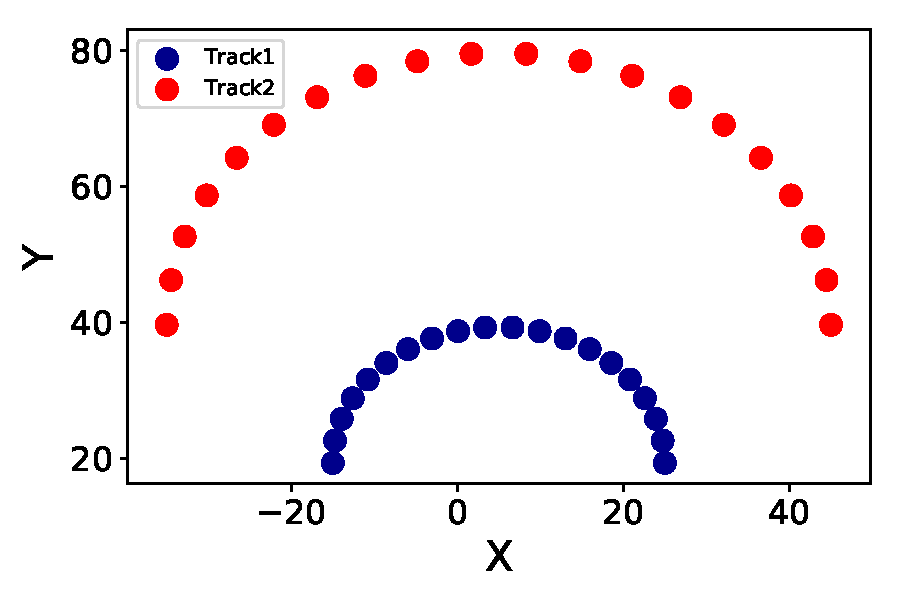
\includegraphics[width=\textwidth]{figures/circle.pdf}
        \caption{}

    \end{subfigure}
		~ %
		\begin{subfigure}[b]{0.3\textwidth}
					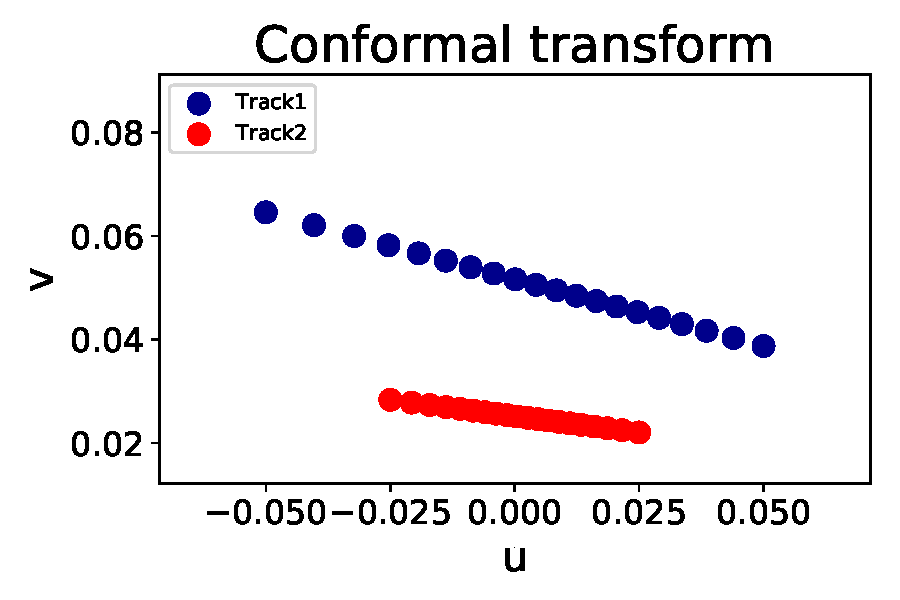
\includegraphics[width=\textwidth]{figures/circle_CT.pdf}
					\caption{}
			\end{subfigure}
			~ %
			\begin{subfigure}[b]{0.3\textwidth}
						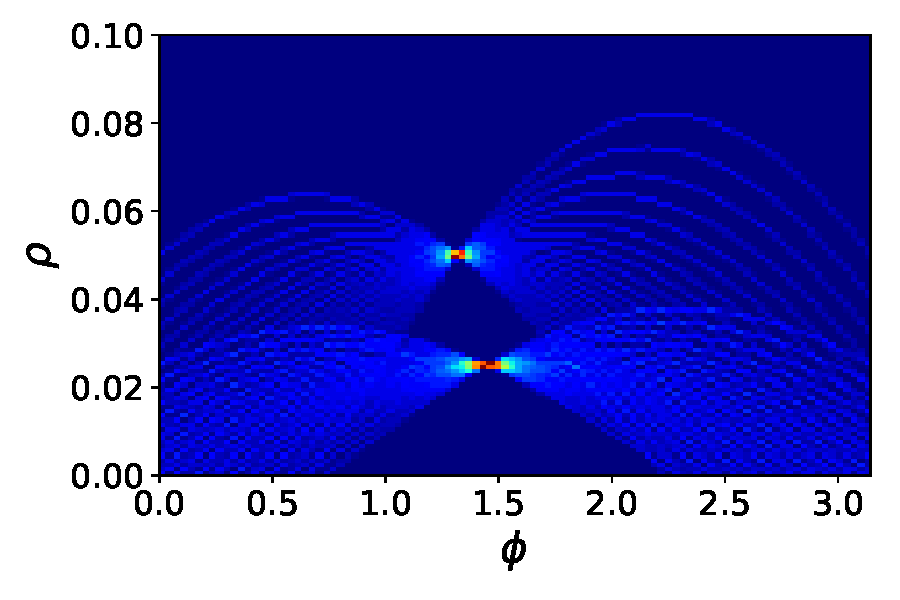
\includegraphics[width=\textwidth]{figures/circle_HT.pdf}
						\caption{}
				\end{subfigure}
	\label{HTcircle}
	\caption{Circles (a) as represented after a conformal mapping (b) and after the Hough transformation (c).}
\end{figure}

The Hough transformation is a periodic function and the points in the $\rho-\theta$ plane are bounded by $\theta \in \left[0, 2\pi\right]$ and $\rho \in \left[-\sqrt{u^2+v^2}, \sqrt{u^2+v^2}\right]$. It is important to note that the points $(\theta, \rho)$ and $(\theta+\pi, -\rho)$ describe the same line. In the studies presented in this document, to remove the ambiguity, $\rho$ is limited to positive values.



\subsection{Identification of single tracks}
The detection of single particle tracks simulated with FCCSW has been investigated.

Simulations using a $2.4\,\gev$ muon particle gun have been done. In a 2~T magnetic field, the bending radius is 4~m. An event is displace in \cref{fig_pgun_3d}.

\begin{figure}[ht]
	\centering
	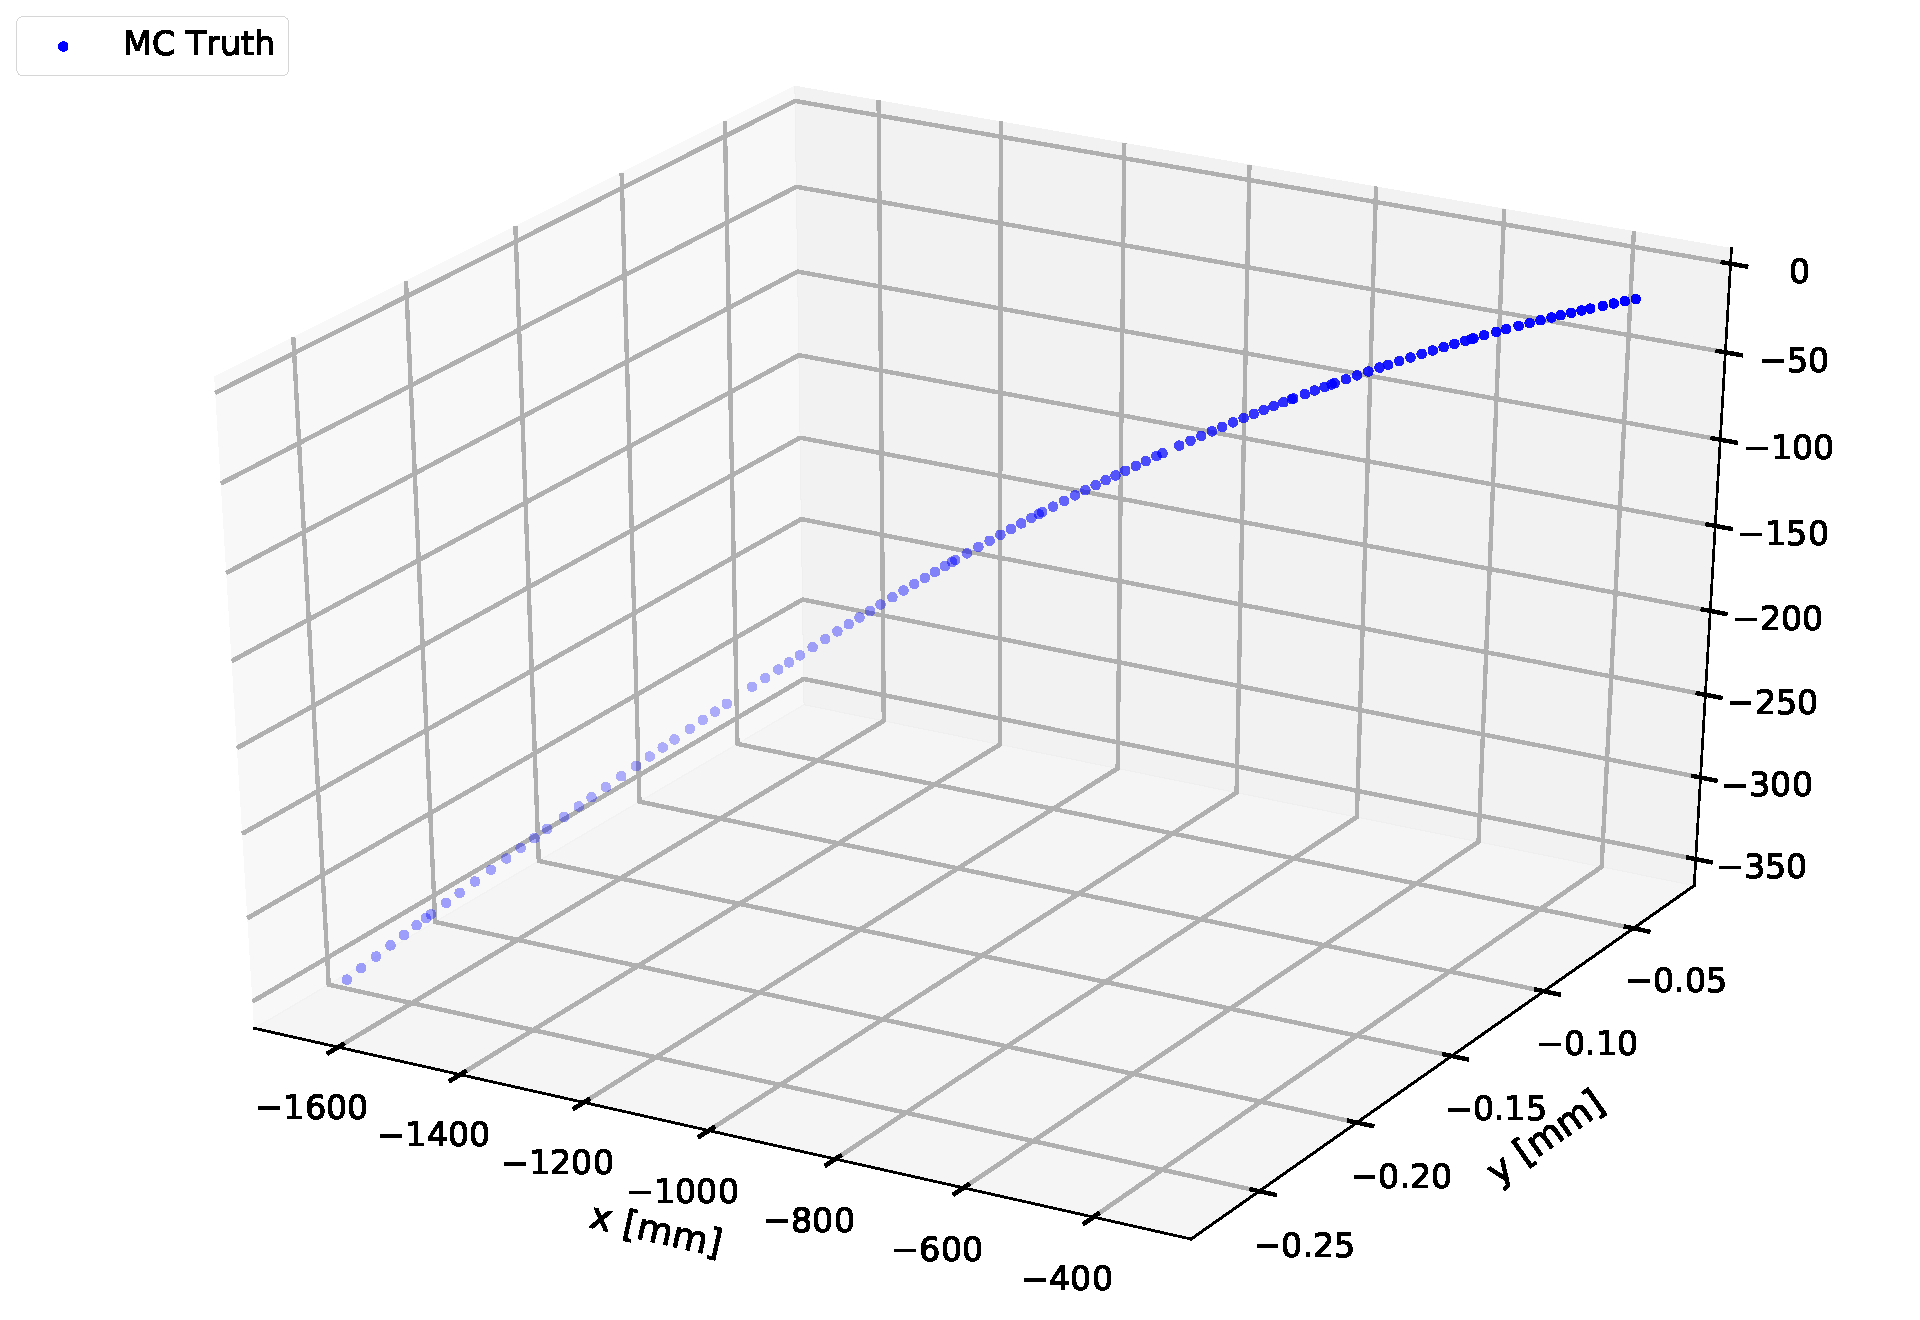
\includegraphics[width=0.6\textwidth]{figures/3D_pgun.pdf}%
	\caption{Simulated hits in the drift chamber for a $2.4\,\gev$ muon in a 2~T magnetic field.}
	\label{fig_pgun_3d}
\end{figure}

\cref{fig_pgun_CT} shows the conformal transformation to the (x-y) position of the simulated hits in the drift chamber and the hits are mapped to a line.

\begin{figure}[ht]
	\centering
	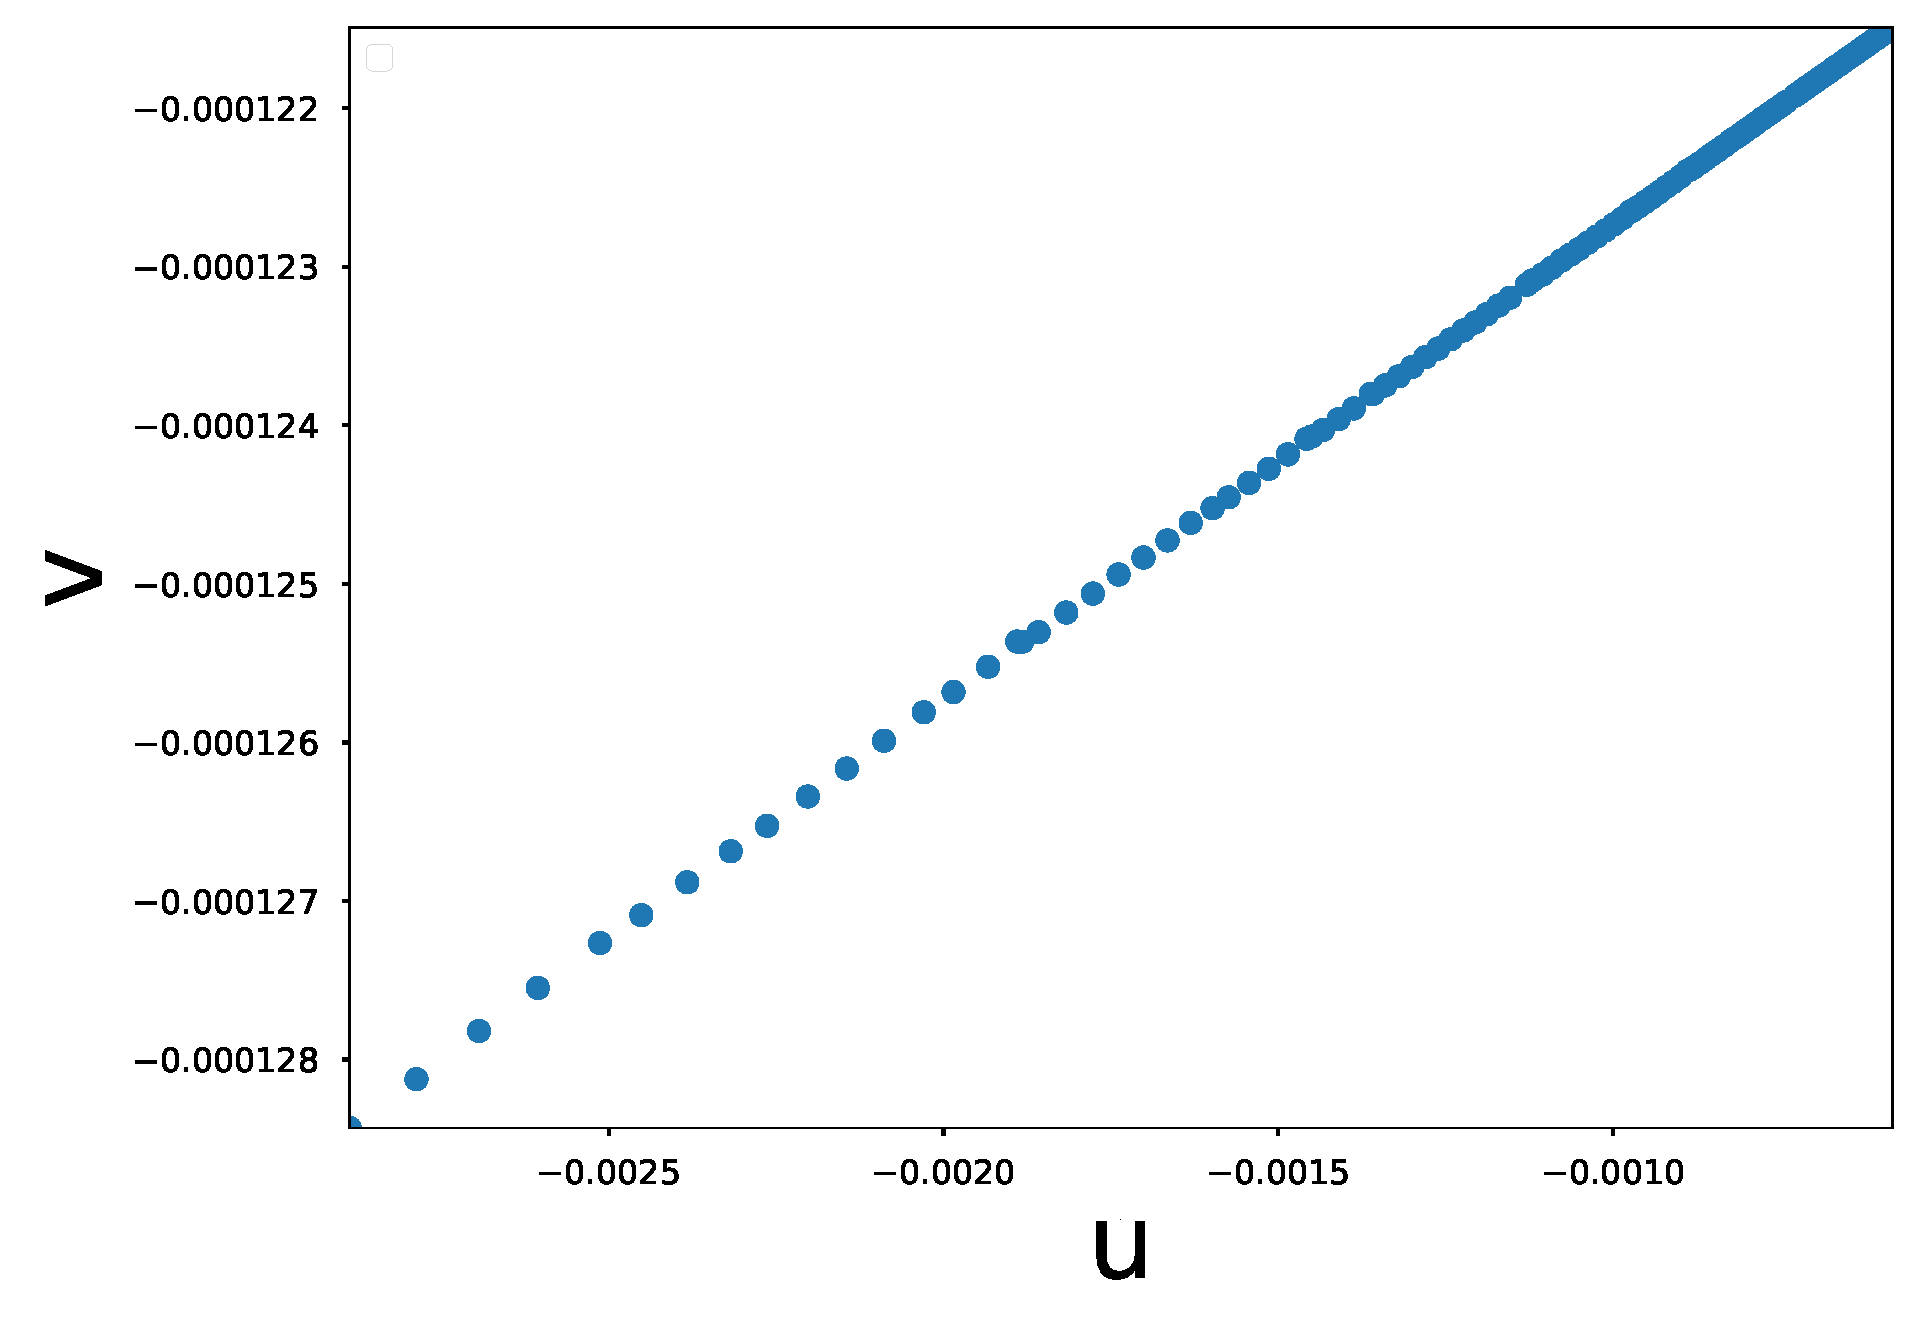
\includegraphics[width=0.6\textwidth]{figures/CT_pgun.pdf}%
	\caption{Conformal transformation for the hits as shown in \cref{fig_pgun_3d}.}
	\label{fig_pgun_CT}
\end{figure}

Finally the Hough transformation is applied to the conformal transform (\cref{fig_pgun_CT}) and the result is shown in \cref{fig_pgun_HT}. In the Hough space, all the hits corresponding to the same track are represented by a local maximum. Therefore, tracks are found by searching for local maxima in the Hough space. Also, the location of the maxima gives the information on the bending radius of the track and its $\phi$-direction.

\begin{figure}[ht]
	\centering
	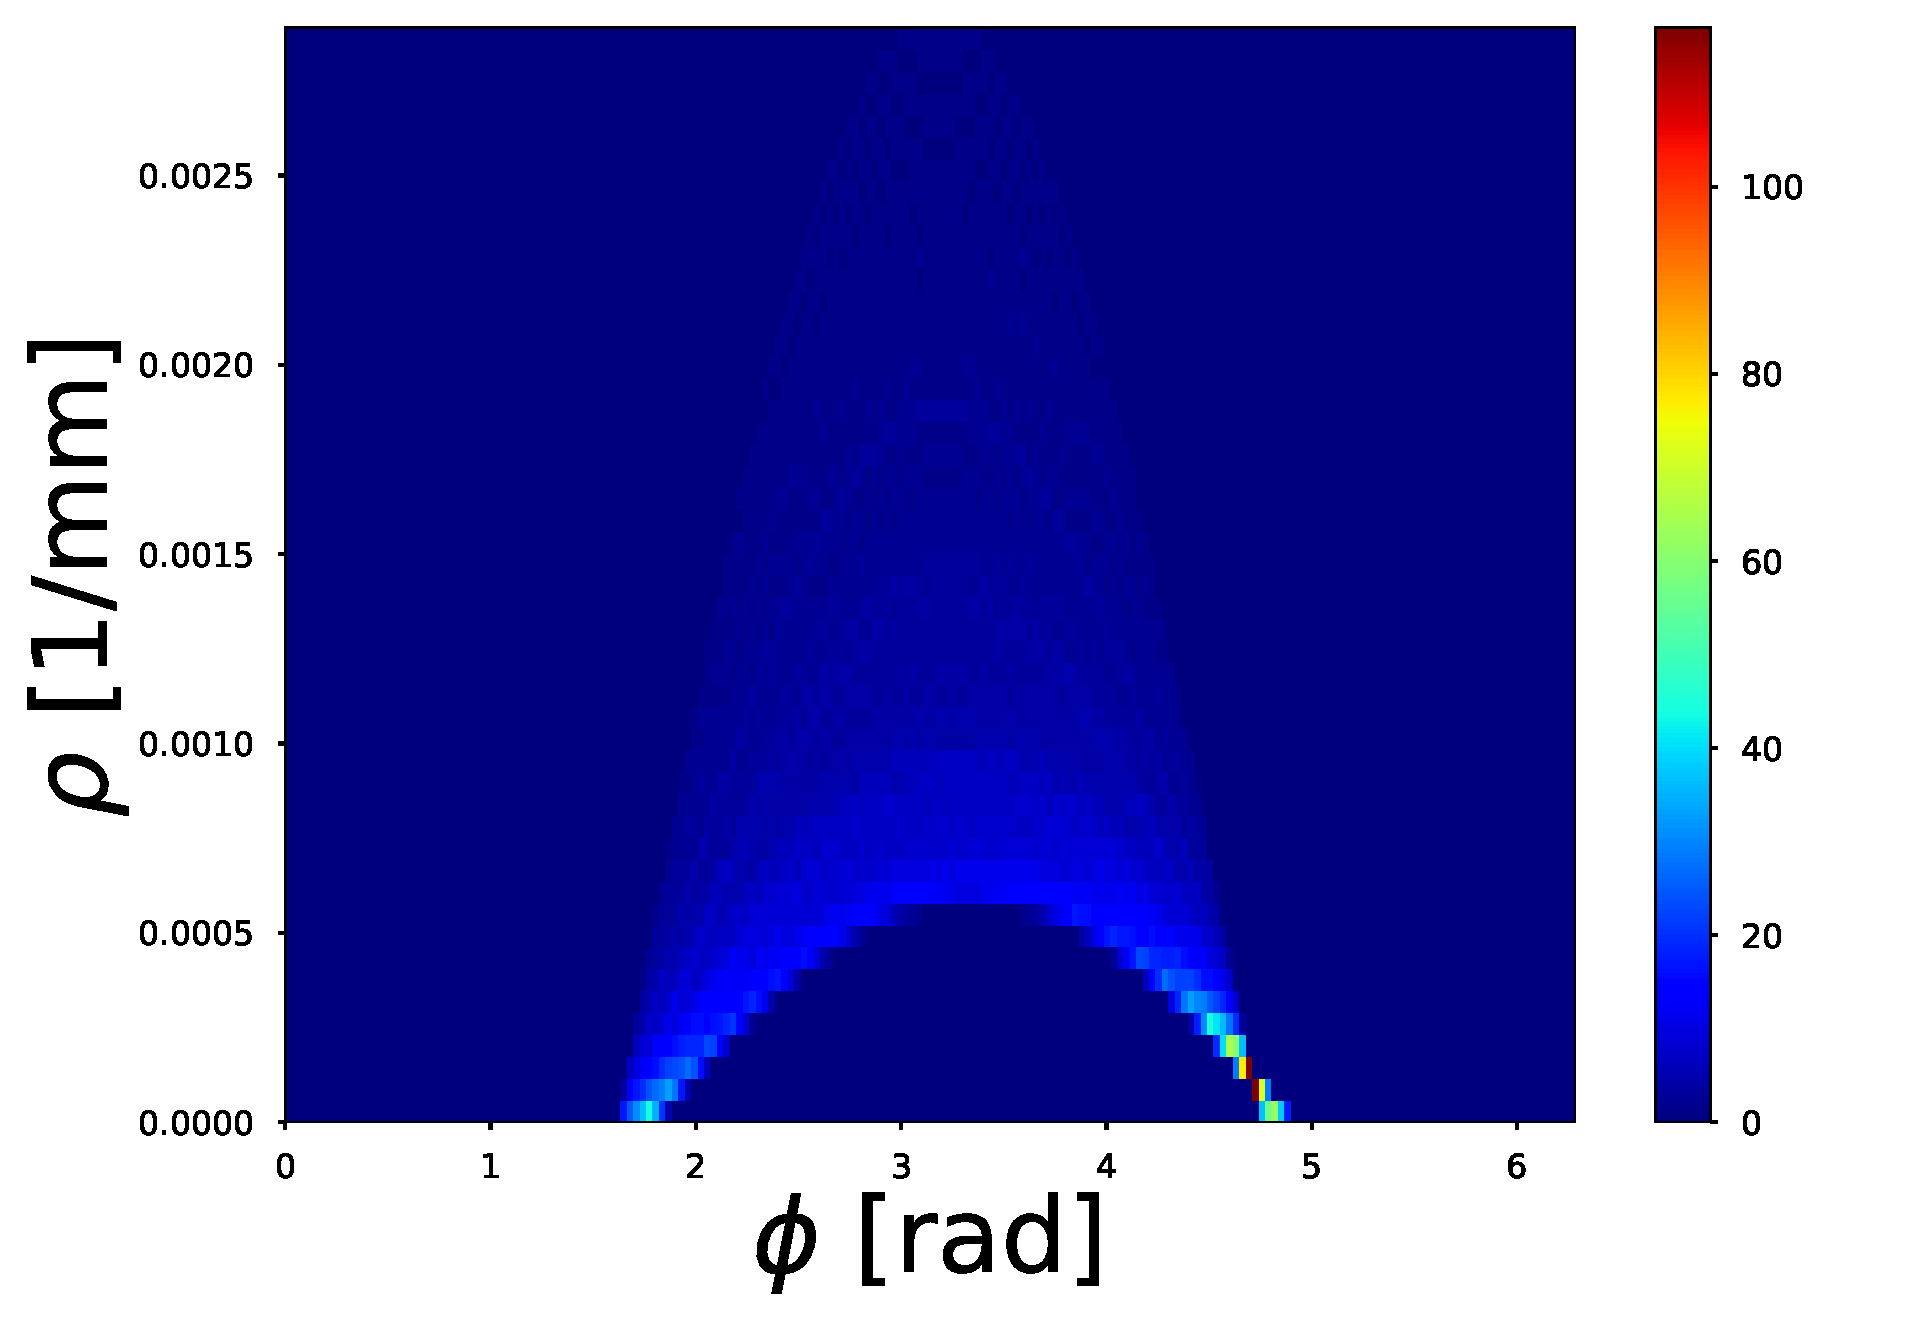
\includegraphics[width=0.6\textwidth]{figures/HT_pgun.pdf}%
	\caption{Hough transformation applied to the conformal transform as shown in \cref{fig_pgun_CT}.}
	\label{fig_pgun_HT}
\end{figure}

\subsection{Finding local maxima in the Hough space}
As seen in the previous chapter, the pattern recognition is performed by looking for local maxima in the Hough space. Since the drift chamber has 112 layers, a threshold is applied to select bins in the Hough space which have more than 112 entries. And to increase the accuracy, the neighboring bins around the bins with maximum hits are also investigated and they are clustered together. \cref{fig_pgun_HT_maxima} shows the bins with at least 112 hits and also one cluster is found. The bending radius of the $2.4\,\gev$ is correctly given by the Hough transformation.

The DBSCAN clustering algorithm\footnote{https://scikit-learn.org/stable/modules/generated/sklearn.cluster.DBSCAN.html} provided by the python library scikit-learn is used with a distance metric. With a distance of $\sqrt{2} \times$~bin size, the clusters' shapes are illustrated in \cref{fig_clushape}.

\begin{figure}[ht]
	\centering
	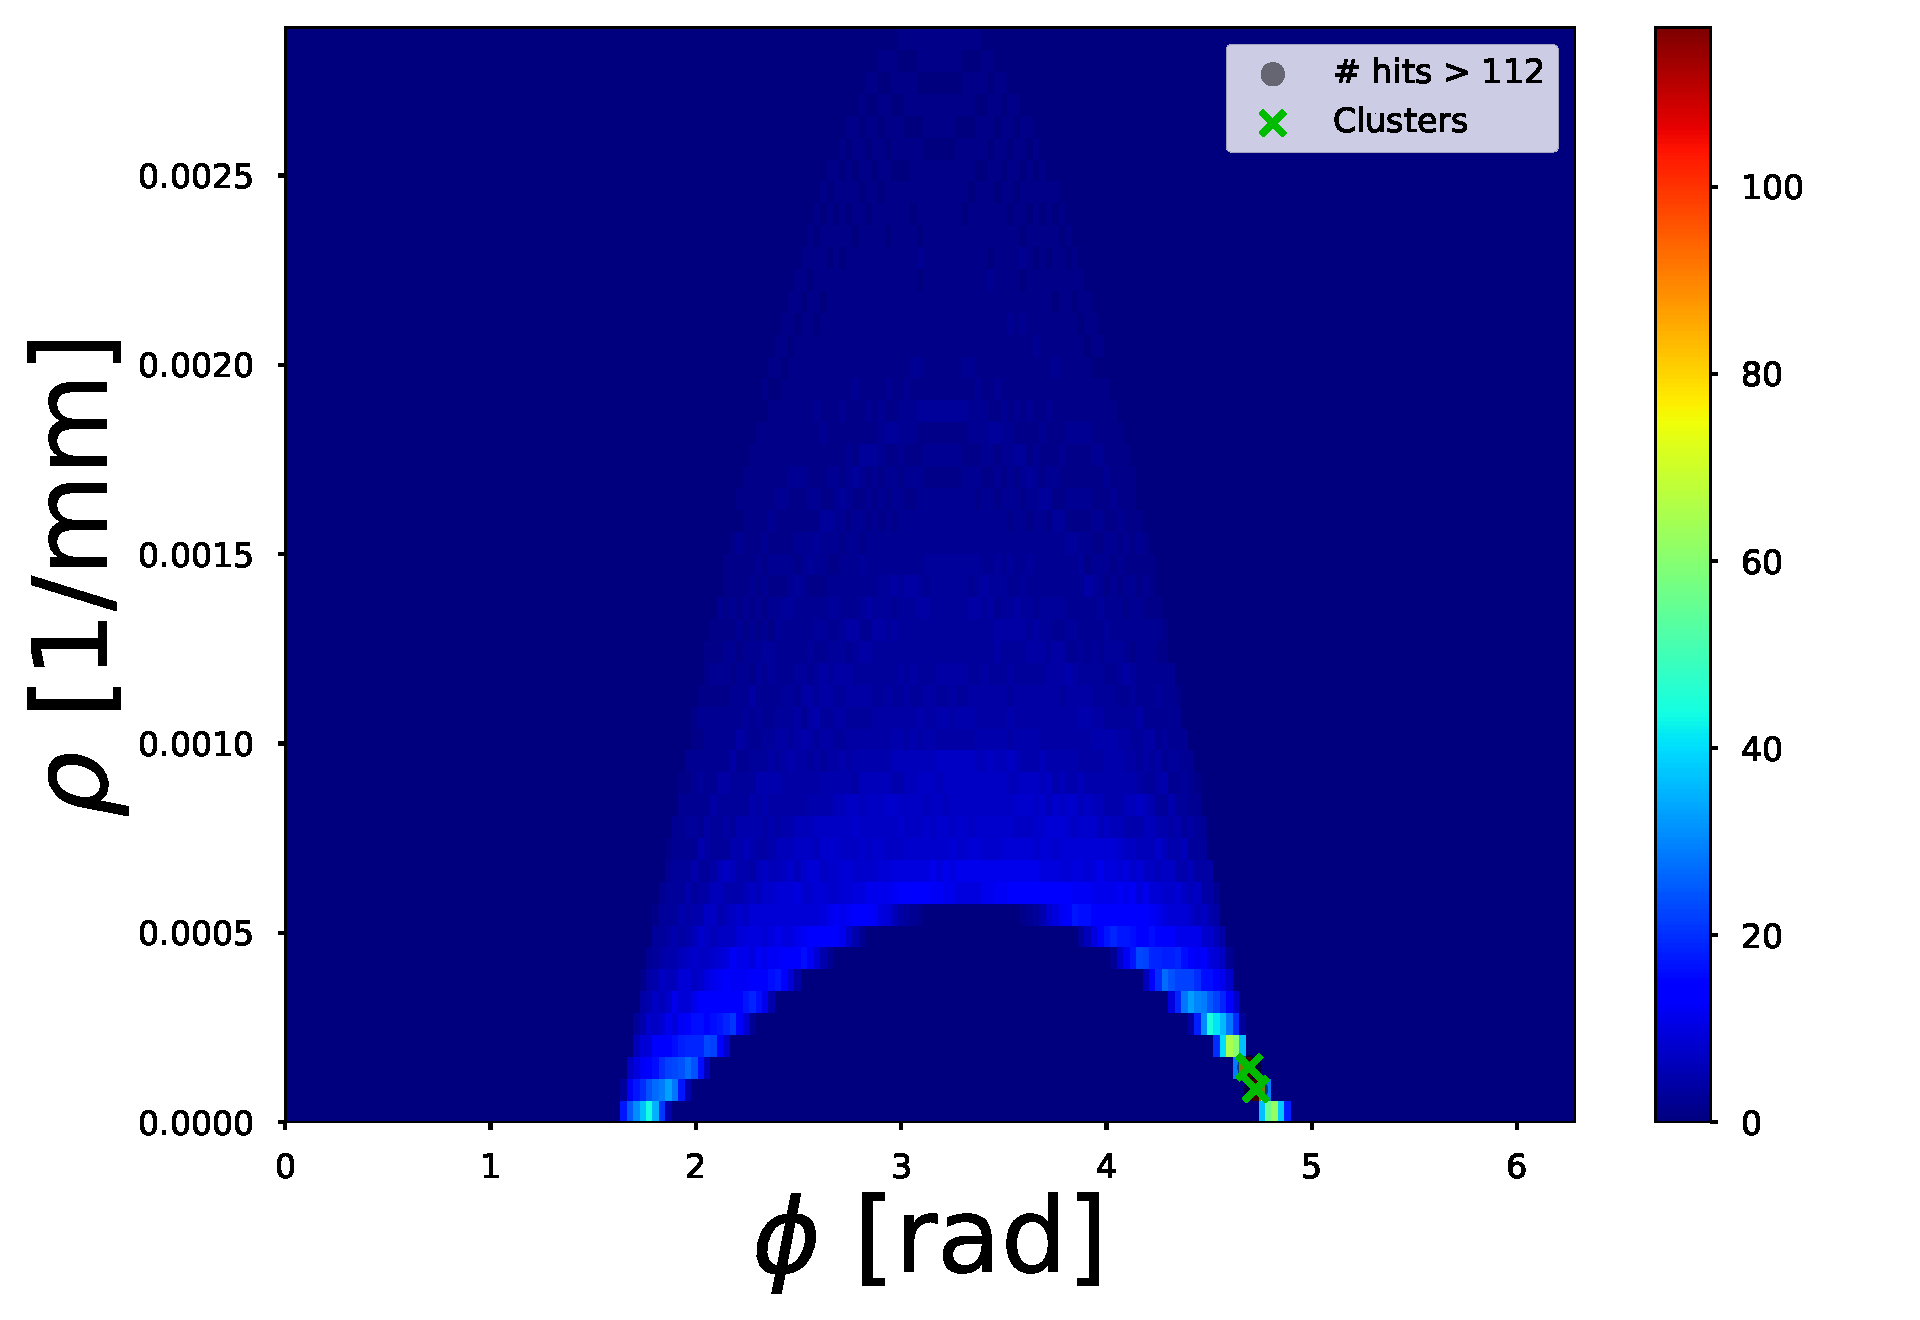
\includegraphics[width=0.6\textwidth]{figures/HT_pgun_maxima.pdf}%
	\caption{Finding the maxima in the Hough space of \cref{fig_pgun_HT}. The bins with more than 112 hits are highlighted and a clustering algorithm is also run.}
	\label{fig_pgun_HT_maxima}
\end{figure}



\begin{figure}[ht]
	\begin{framed}
	\centering
	\begin{subfigure}[b]{0.3\textwidth}
		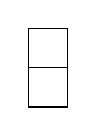
\begin{tikzpicture}
			\draw (0,0) rectangle (0.5, 0.5);
			\draw (0, 0.5) rectangle (00.5, 1);
		\end{tikzpicture}
  \end{subfigure}
		~ %
	\centering
	\begin{subfigure}[b]{0.3\textwidth}
		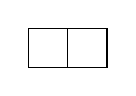
\begin{tikzpicture}
		\draw (0,0) rectangle (0.5, 0.5);
		\draw (0.5, 0) rectangle (1, 0.5);
		\end{tikzpicture}
		\end{subfigure}
			~ %
	\centering
	\begin{subfigure}[b]{0.3\textwidth}
		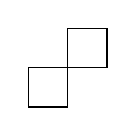
\begin{tikzpicture}
      \draw (0,0) rectangle (0.5, 0.5);
      \draw (0.5, 0.5) rectangle (1, 1);
      \end{tikzpicture}
		\end{subfigure}
		\end{framed}
	\label{fig_clushape}
	\caption{Configurations where the shapes are considered as a cluster with a distance criterion of $\sqrt{2}$.}
\end{figure}


\subsection{Incoherent $e^+e^-$ background pairs}

\cref{fig_bcg} shows the simulated hits in the drift chamber due to incoherent $e^+e^-$ background pairs.

\begin{figure}[ht]
	\centering
	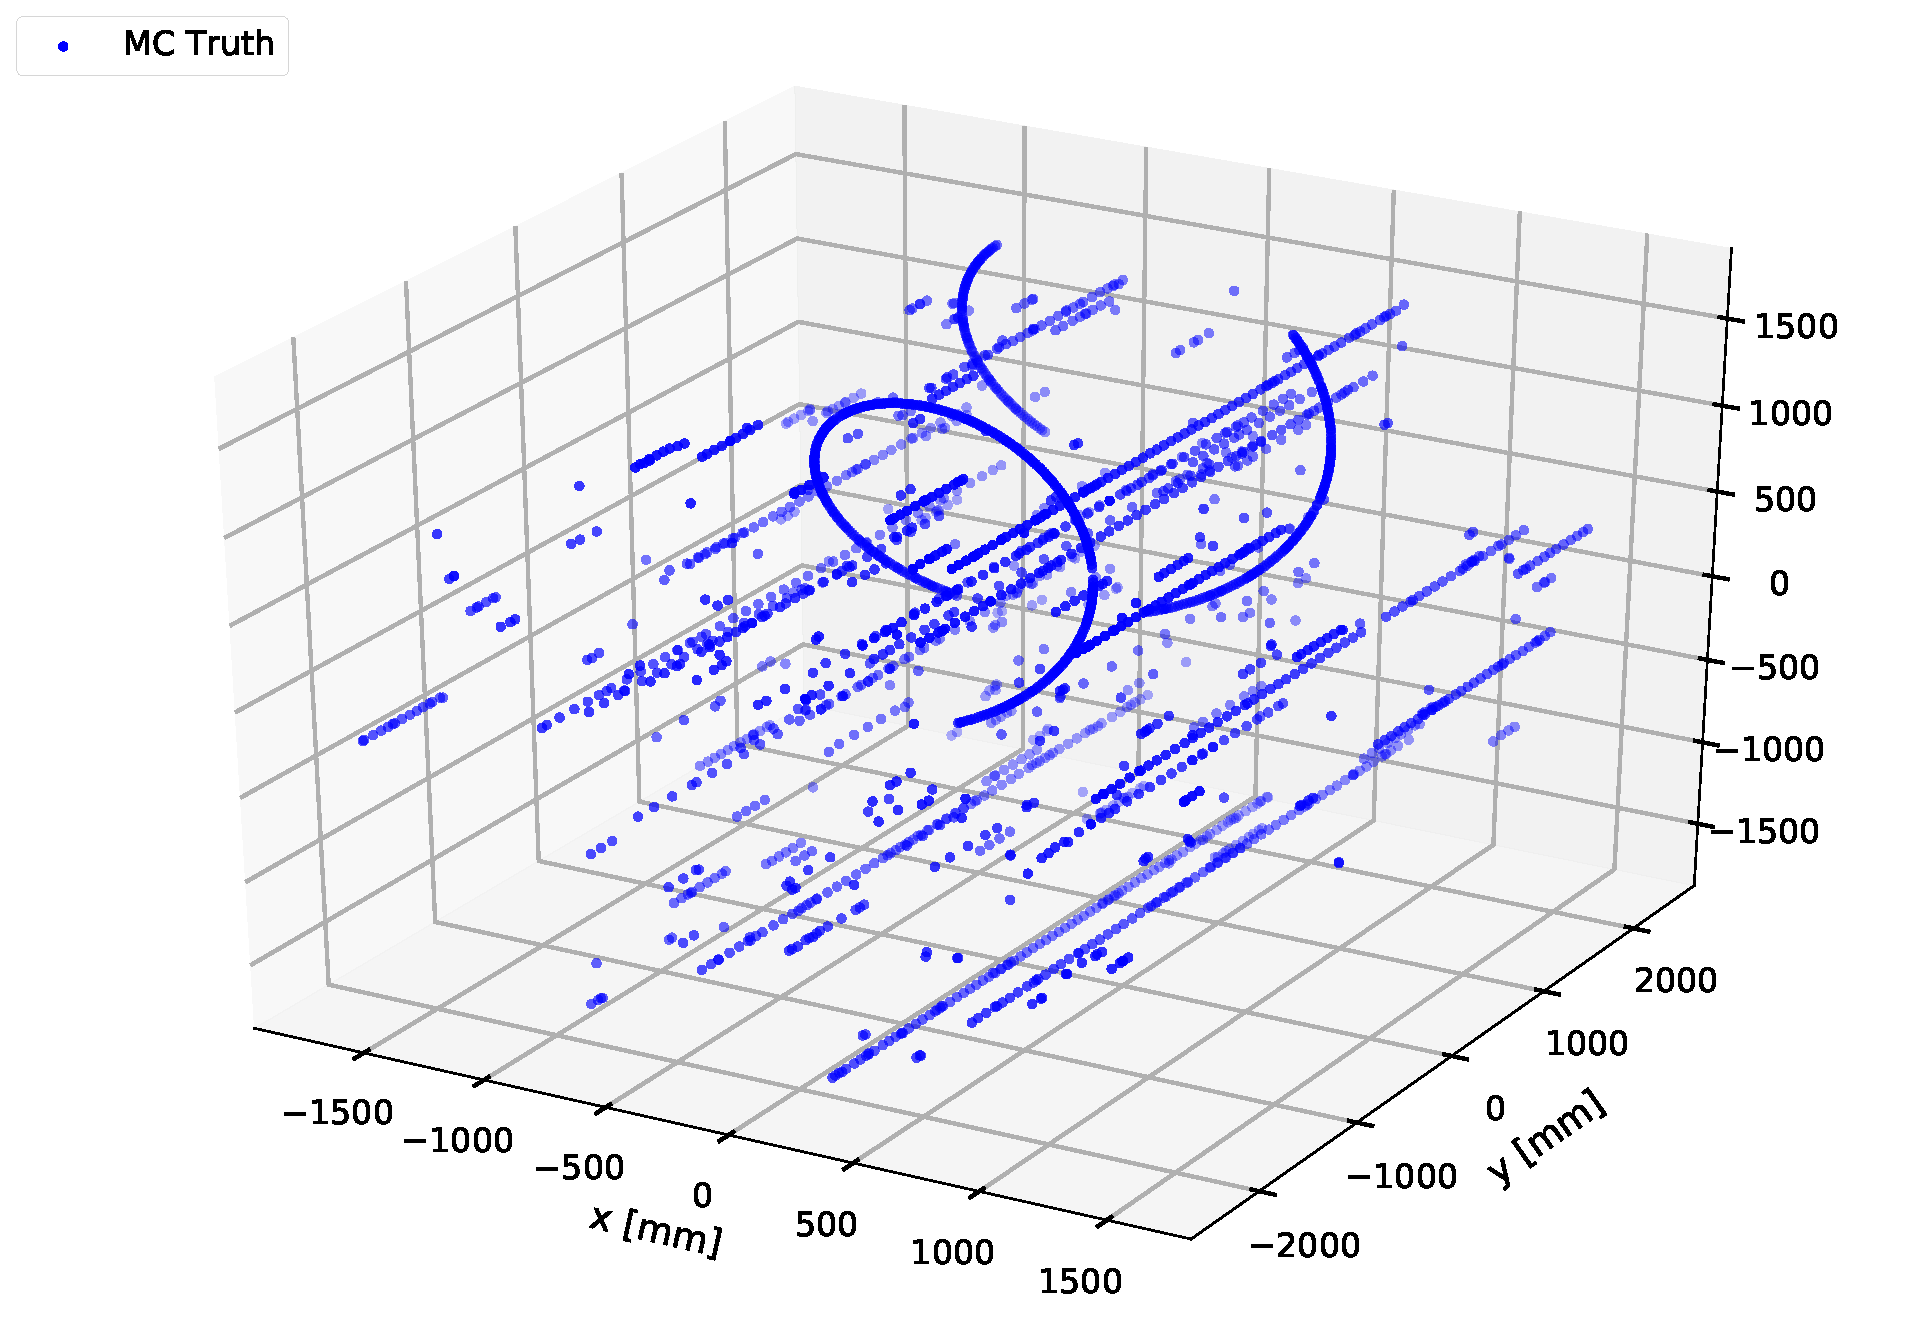
\includegraphics[width=0.6\textwidth]{figures/3D_background.pdf}%
	\caption{Display of the incoherent $e^+e^-$ background hits in the drift chamber.}
	\label{fig_bcg}
\end{figure}

The conformal transformation corresponding to the hits as shown in \cref{fig_bcg} is shown in \cref{fig_bcg_CT}. The conformal transform displays the tracks as lines.

\begin{figure}[ht]
	\centering
	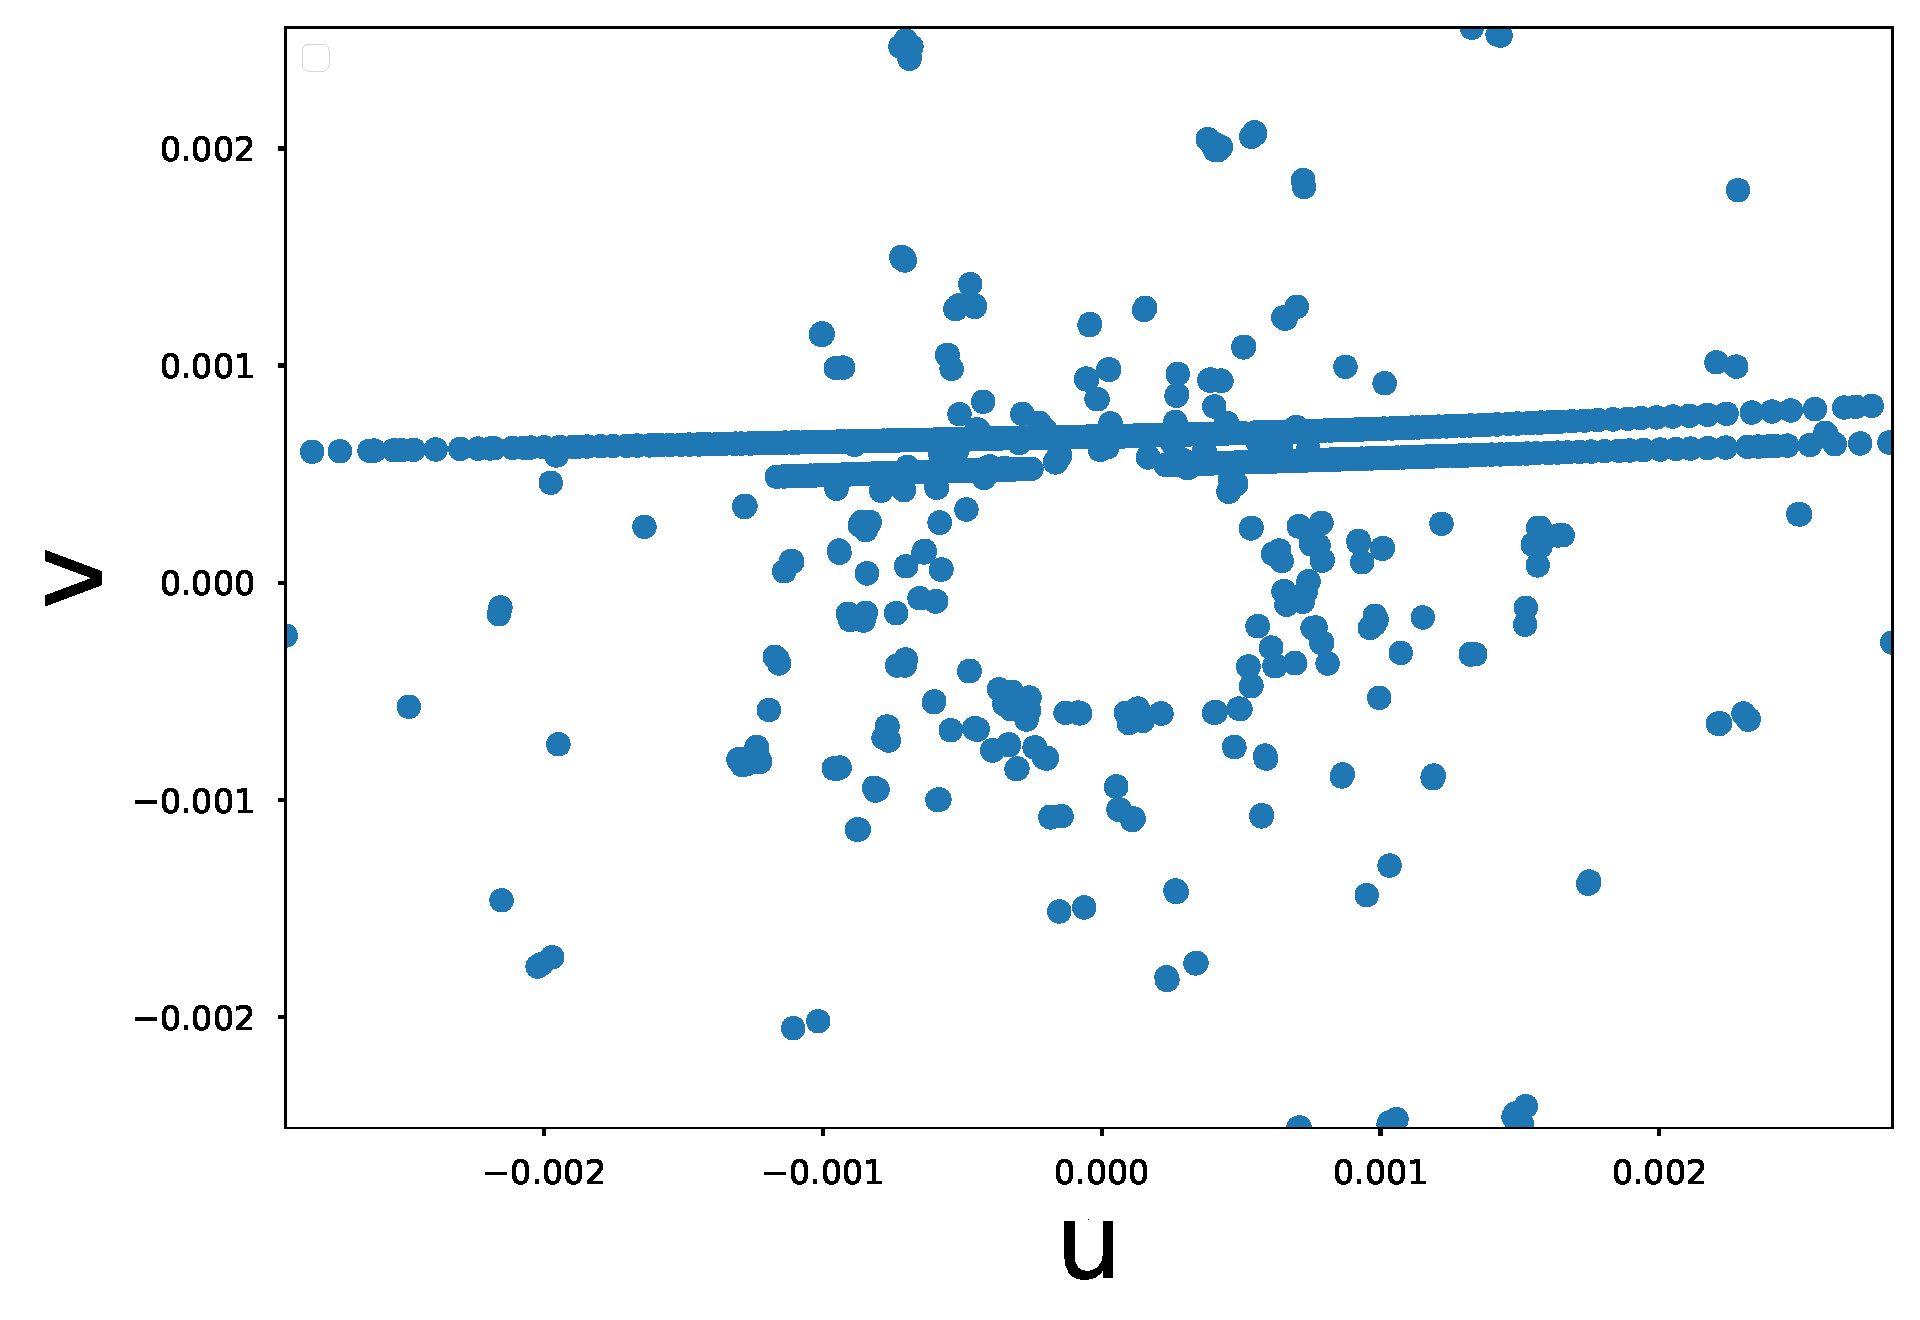
\includegraphics[width=0.6\textwidth]{figures/CT_background.pdf}%
	\caption{Display of the incoherent $e^+e^-$ background hits in the drift chamber.}
	\label{fig_bcg_CT}
\end{figure}

\cref{fig_bcg_HT} shows the Hough transformation of the background hits. The clustering algorithm finds 30 clusters. The confusion is due to the noisy environment. Also, the bin size and the threshold have a high impact on the number of clusters found. To reconstruct tracks in such a noisy environment, two solutions can be explored. First, the timing of the incoherent pairs can be explored to reduce hits with high timings. The second method would be to use the information from the seeding in the vertex detector and restrict the search for tracks in the Hough space based on the seeds.

\begin{figure}[ht]
	\centering
	\begin{subfigure}[b]{0.48\textwidth}
        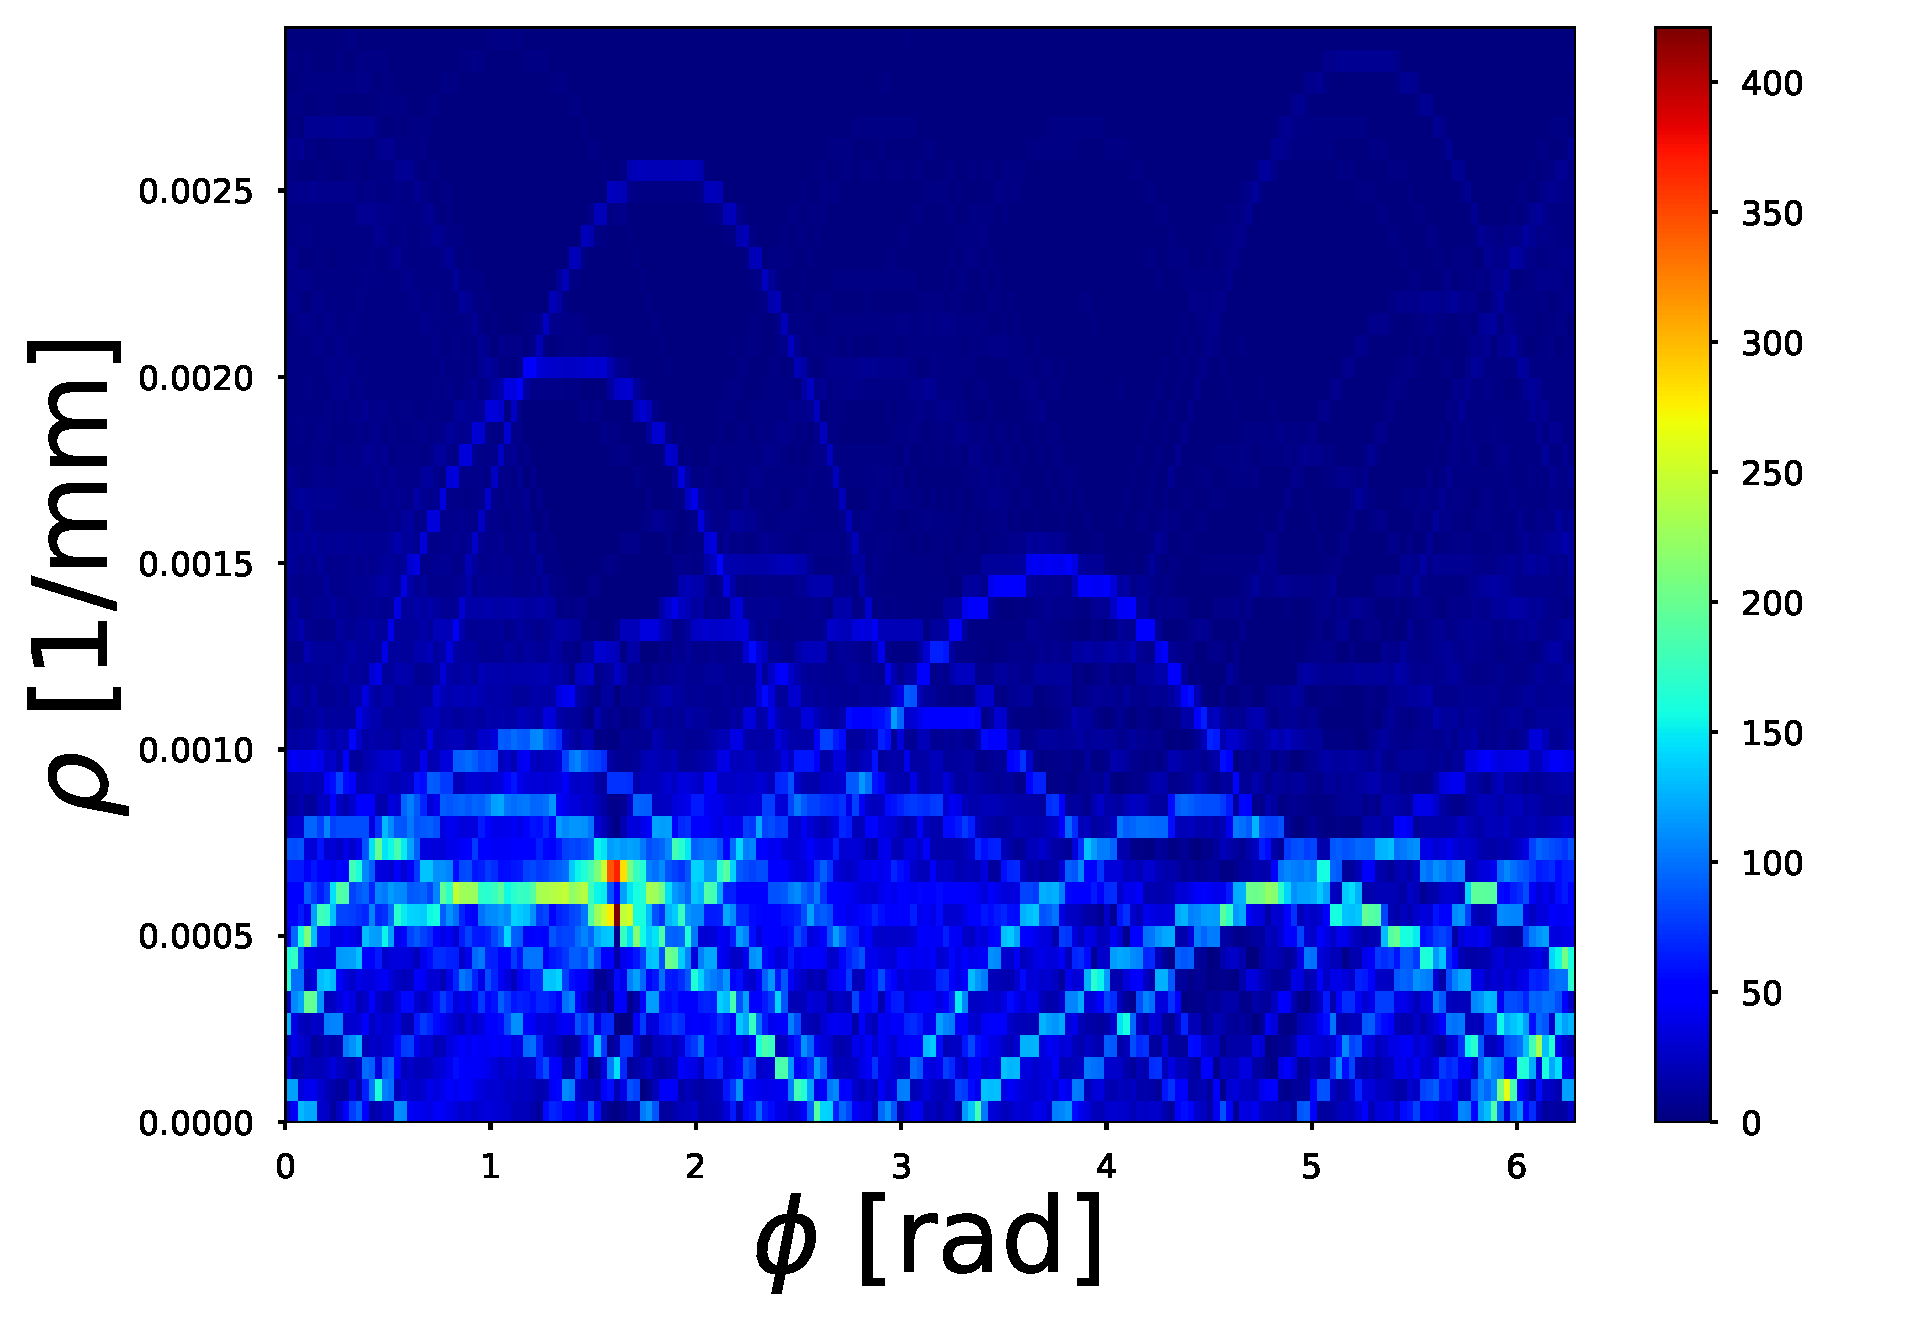
\includegraphics[width=\textwidth]{figures/HT_background.pdf}
        \caption{}

    \end{subfigure}
		~ %
		\begin{subfigure}[b]{0.48\textwidth}
					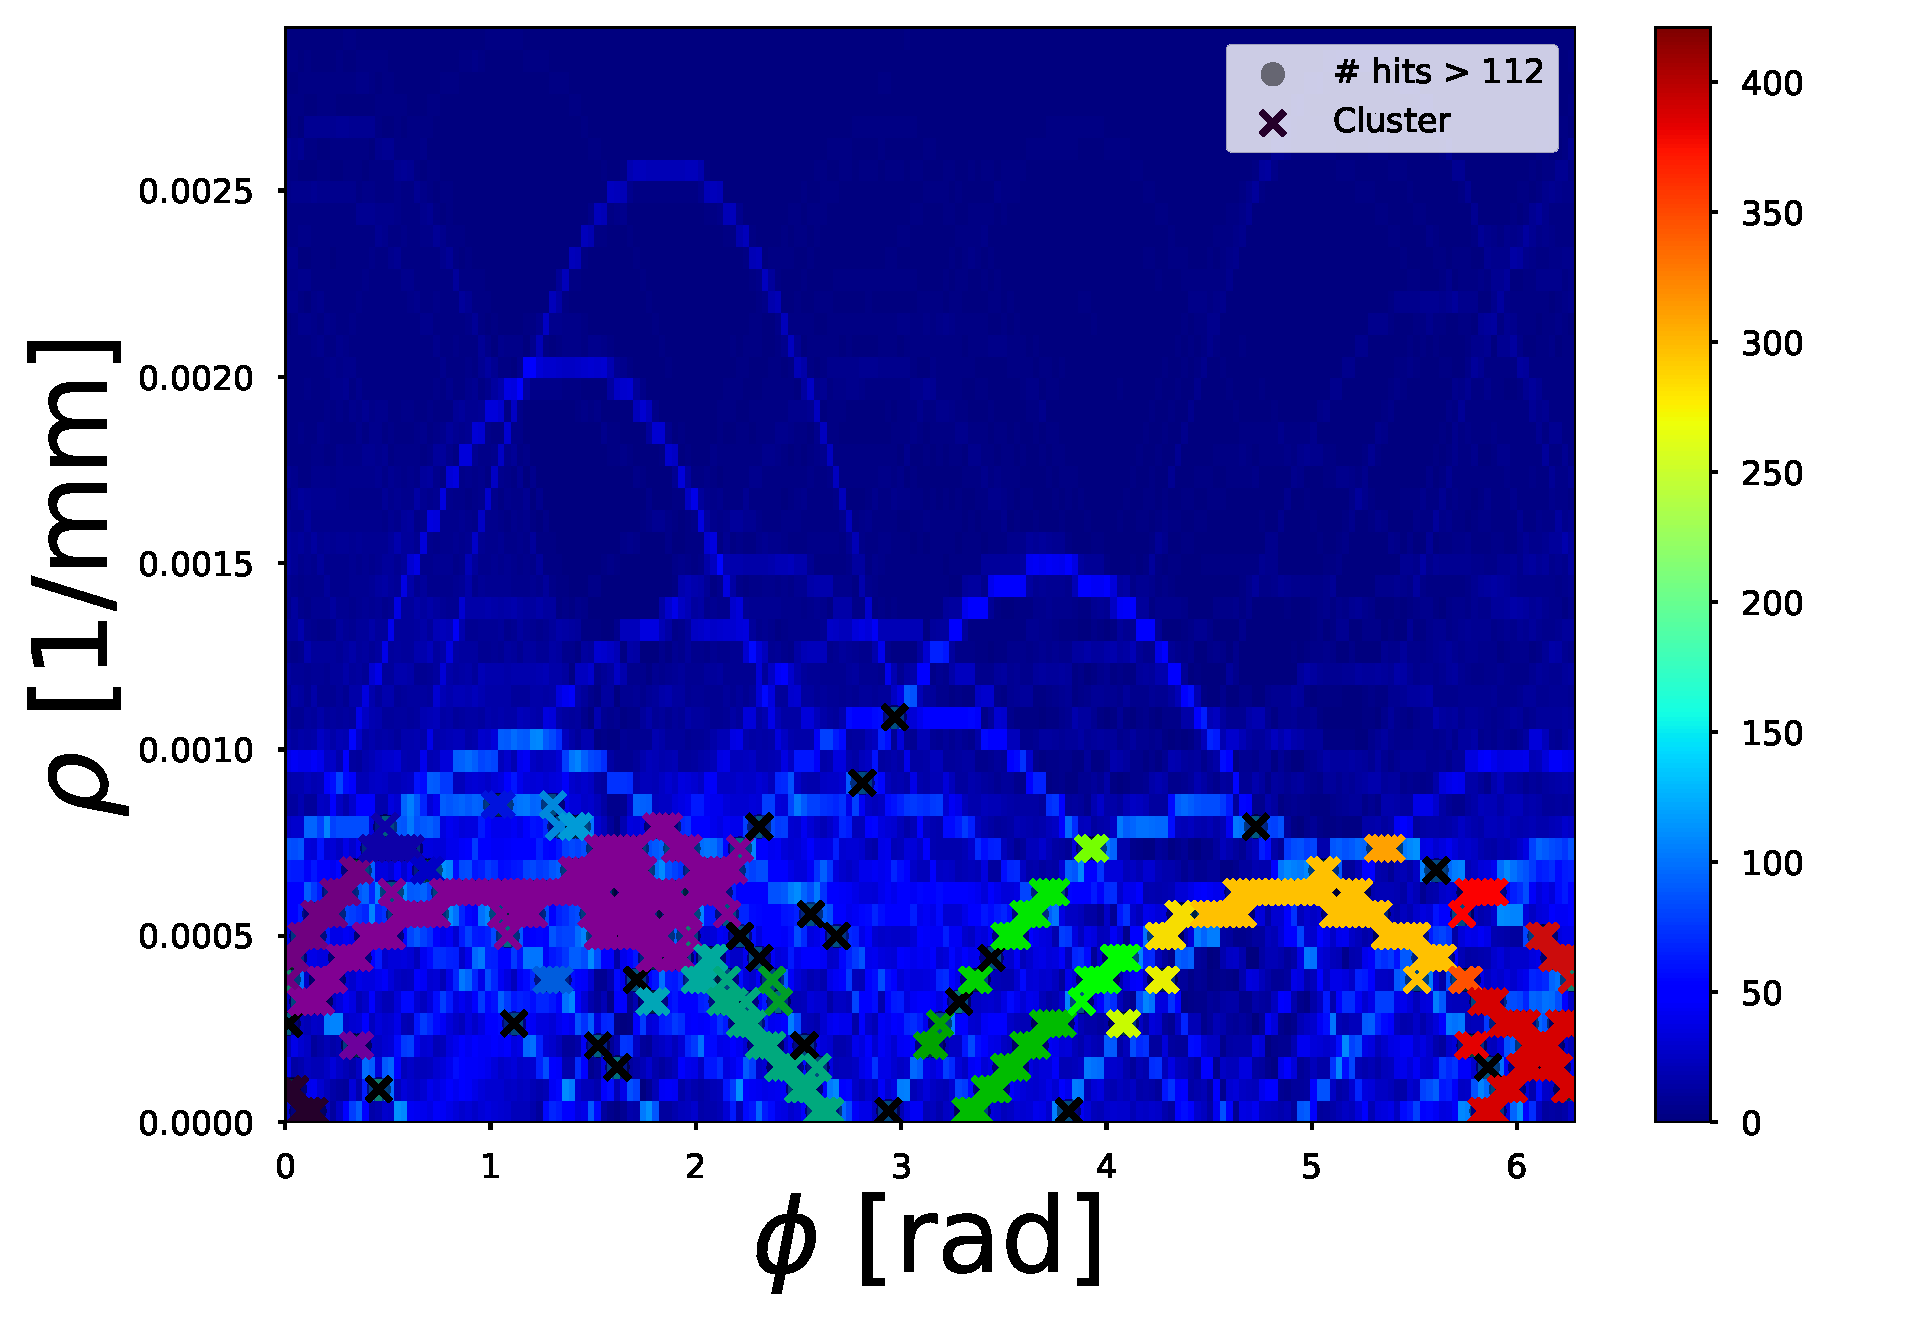
\includegraphics[width=\textwidth]{figures/HT_background_maxima.pdf}
					\caption{}
			\end{subfigure}
	\label{fig_bcg_HT}
	\caption{(a) shows the $e^+e^-$ background hits as represented in the Hough space. (b) shows the clusters found by the clustering algorithm.}
\end{figure}


\subsection{Dijet events}

The Hough transformation is also investigated for more complex events such as the decay of the Z-like boson into two light-quark dijets (Z~$\rightarrow$~d\={d}) for a center-of-mass energy of $\sqrt{s} = 91 \,\gev$.
The hits in the drift chamber are displayed in \cref{fig_Zdd}.

\begin{figure}[ht]
	\centering
	\begin{subfigure}[b]{0.48\textwidth}
        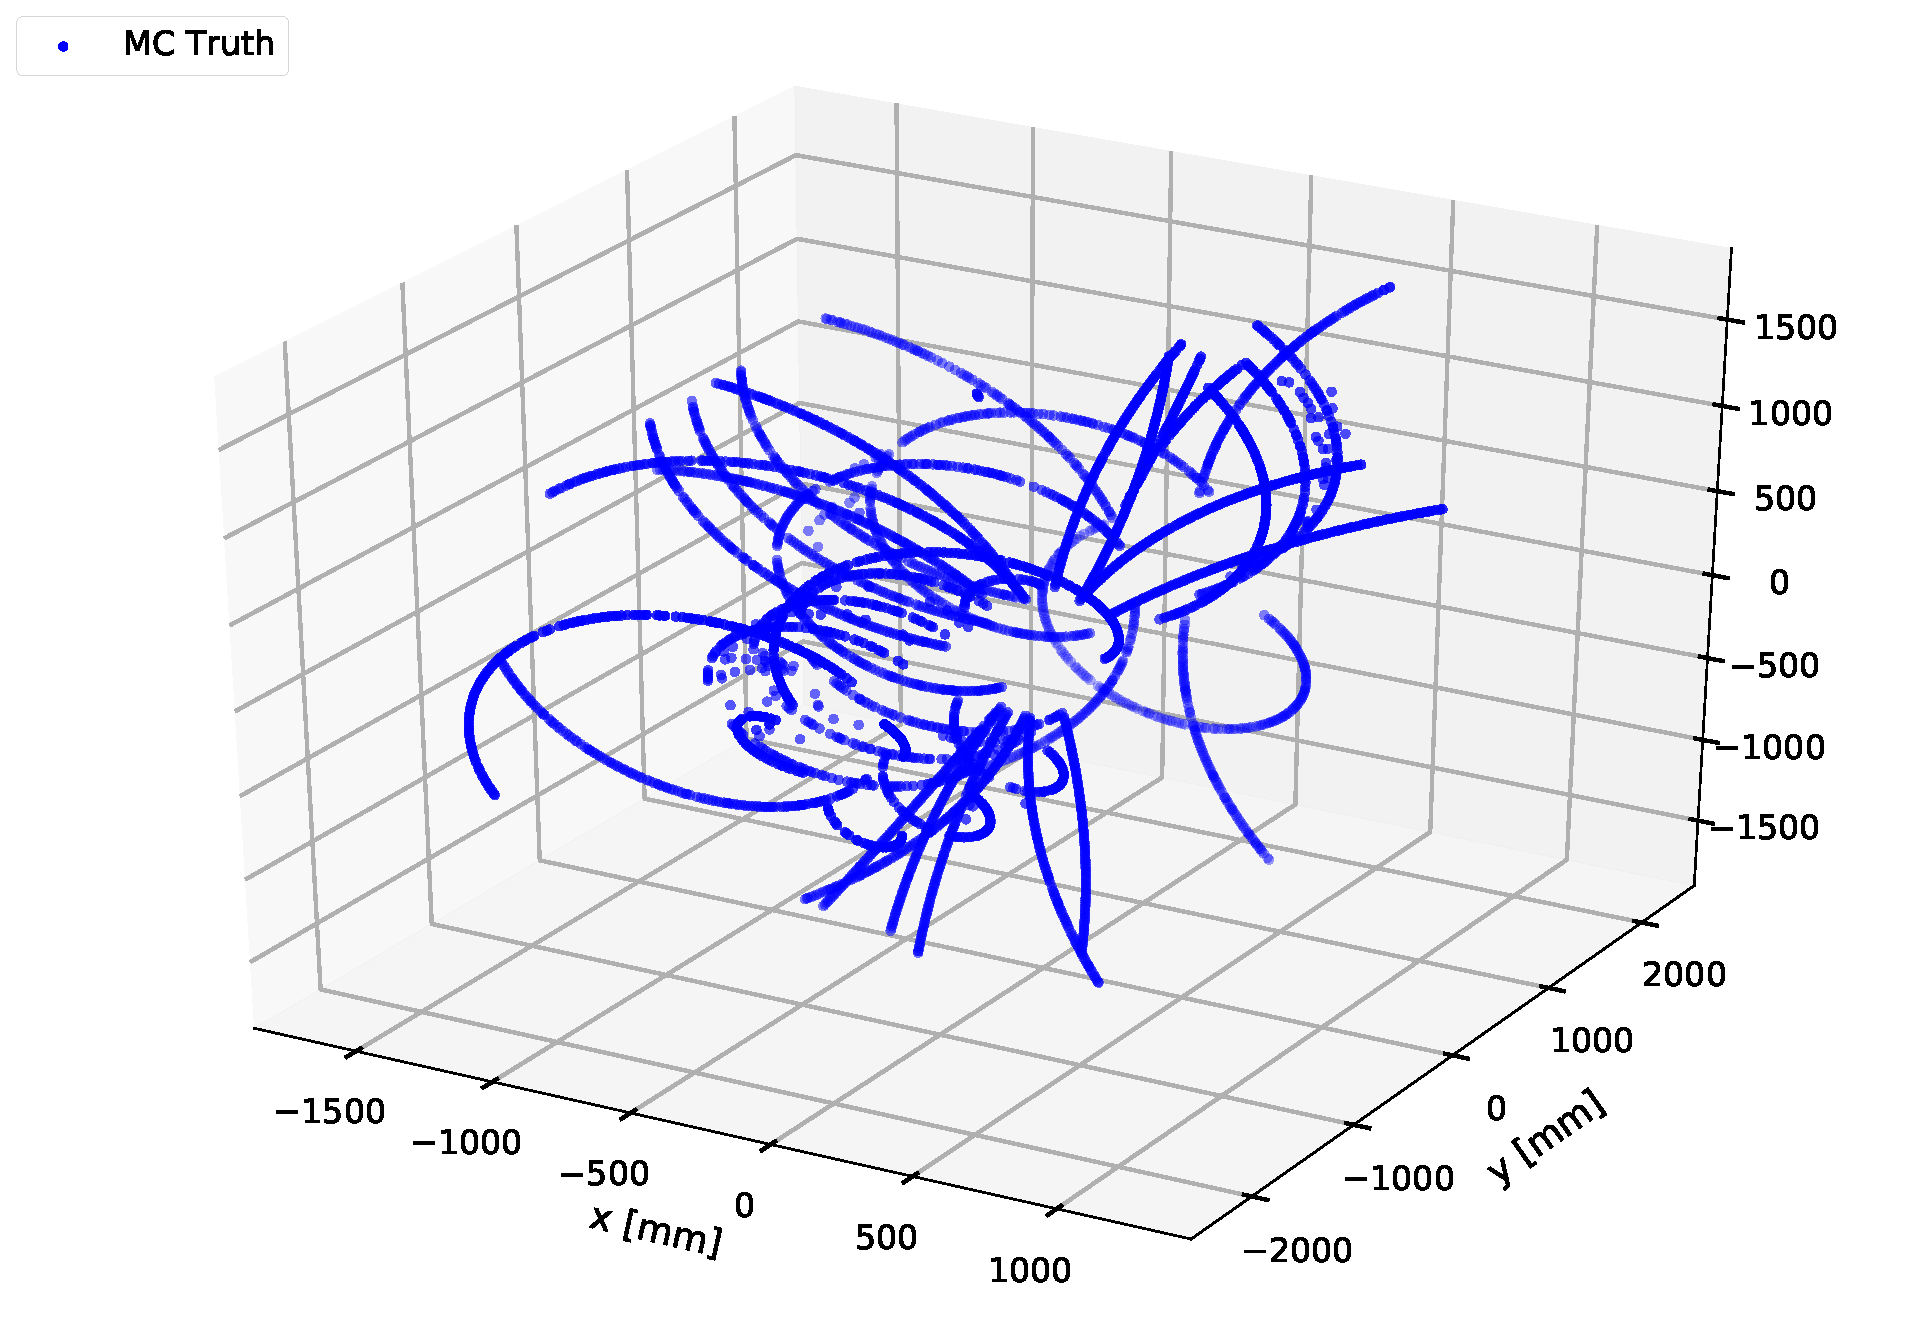
\includegraphics[width=\textwidth]{figures/3D_Zdd.pdf}
        \caption{}
    \end{subfigure}
		~ %
		\begin{subfigure}[b]{0.48\textwidth}
					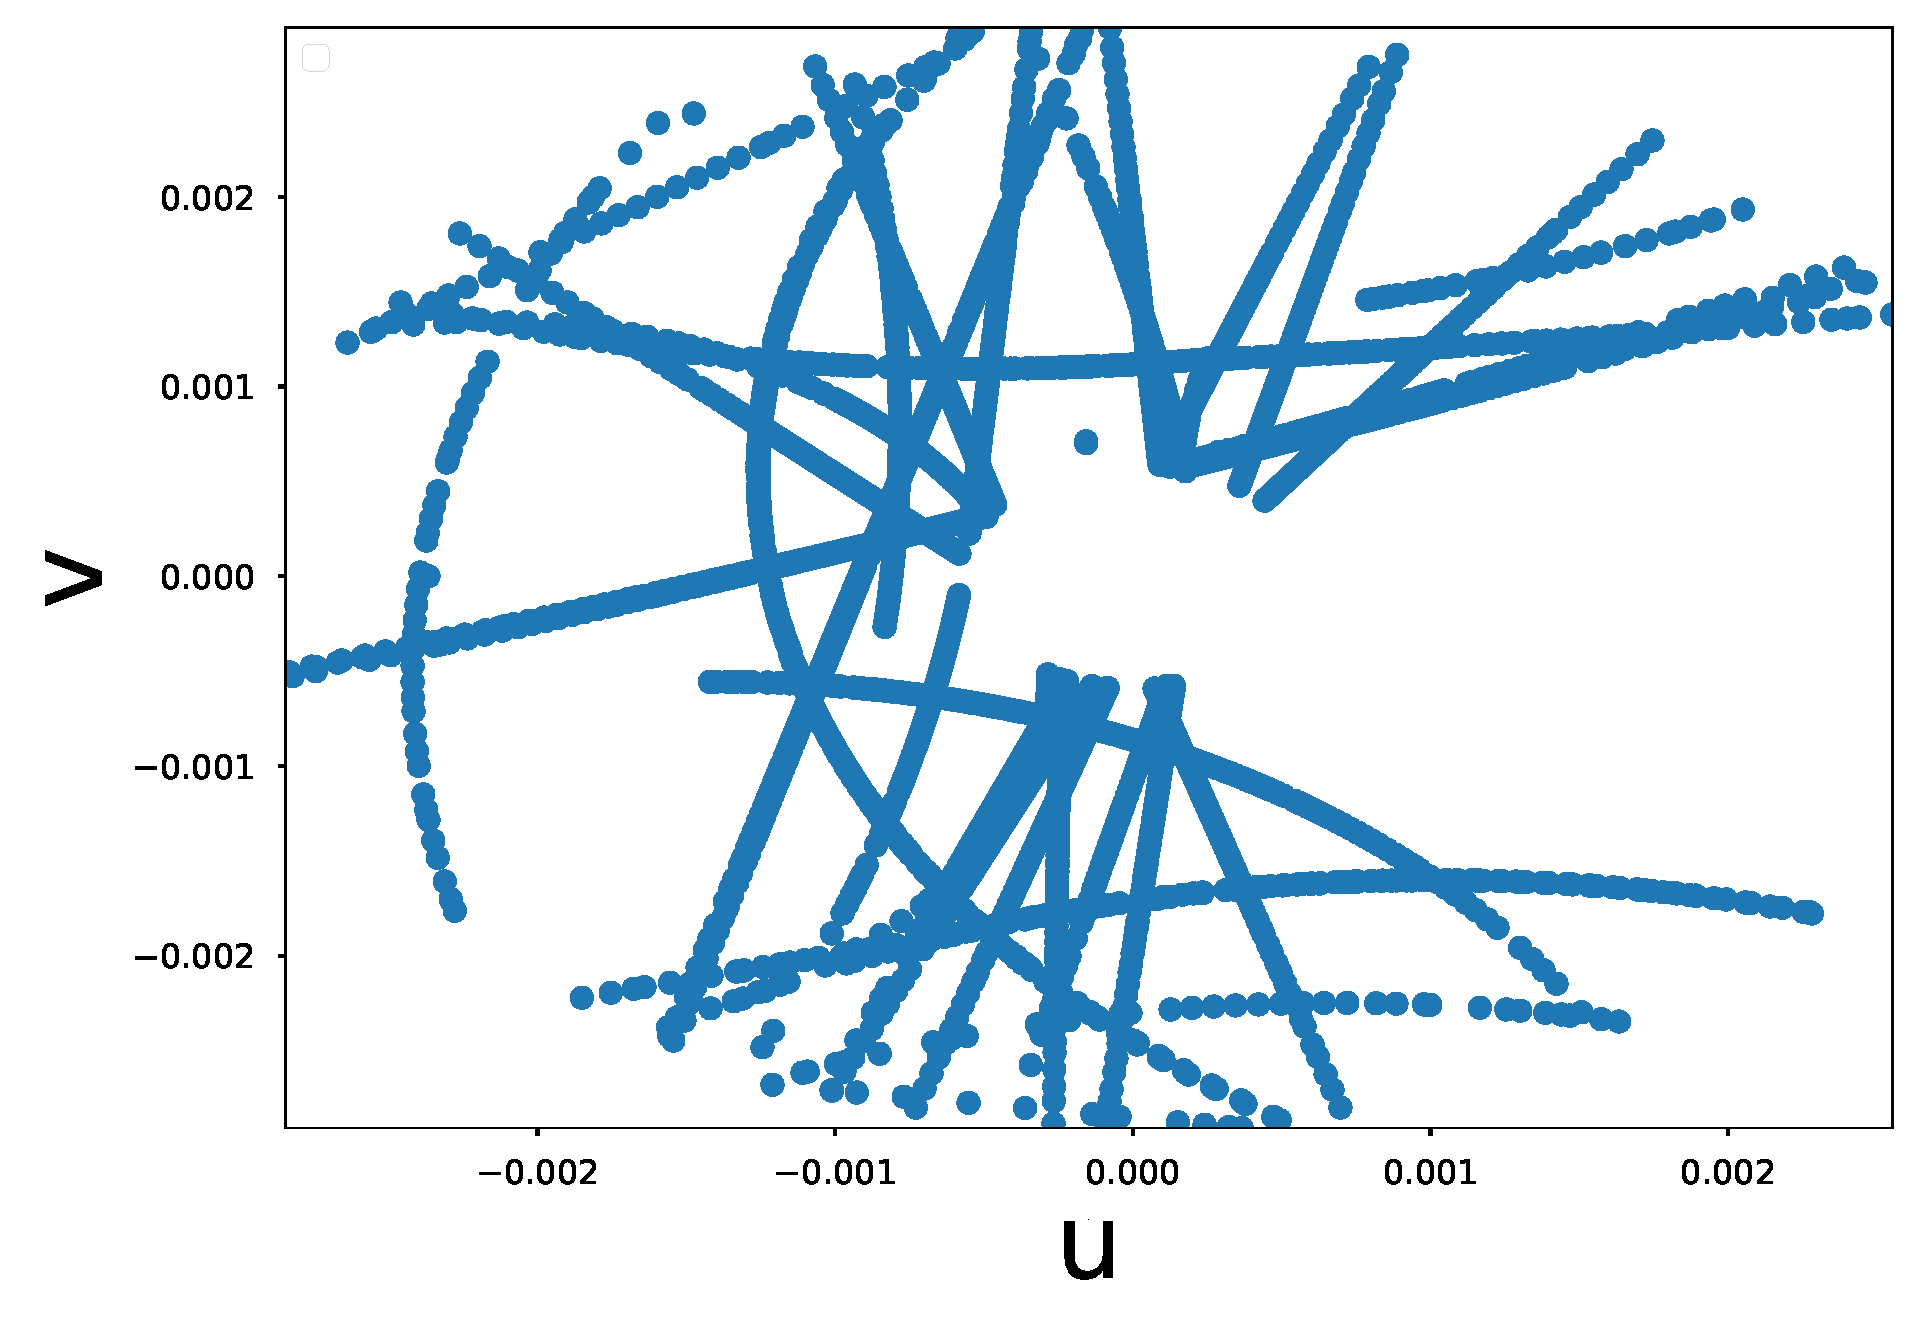
\includegraphics[width=\textwidth]{figures/CT_Zdd.pdf}
					\caption{}
			\end{subfigure}
	\caption{(a) display of the hits in the drift chamber due to the decay Z~$\rightarrow$~d\={d} at a center-of-mass energy of $\sqrt{s} = 91 \,\gev$. (b) displays the conformal transformation of such complex events.}
	\label{fig_Zdd}
\end{figure}

The Hough transformation for such a complex event is shown in \cref{HTZdd}. As seen previously, the clustering can be very sensitive to the threshold and bin sizes in the Hough space. The information from the seeding of the vertex detector can improve the pattern recognition in the drift chamber.

\begin{figure}[ht]
	\centering
  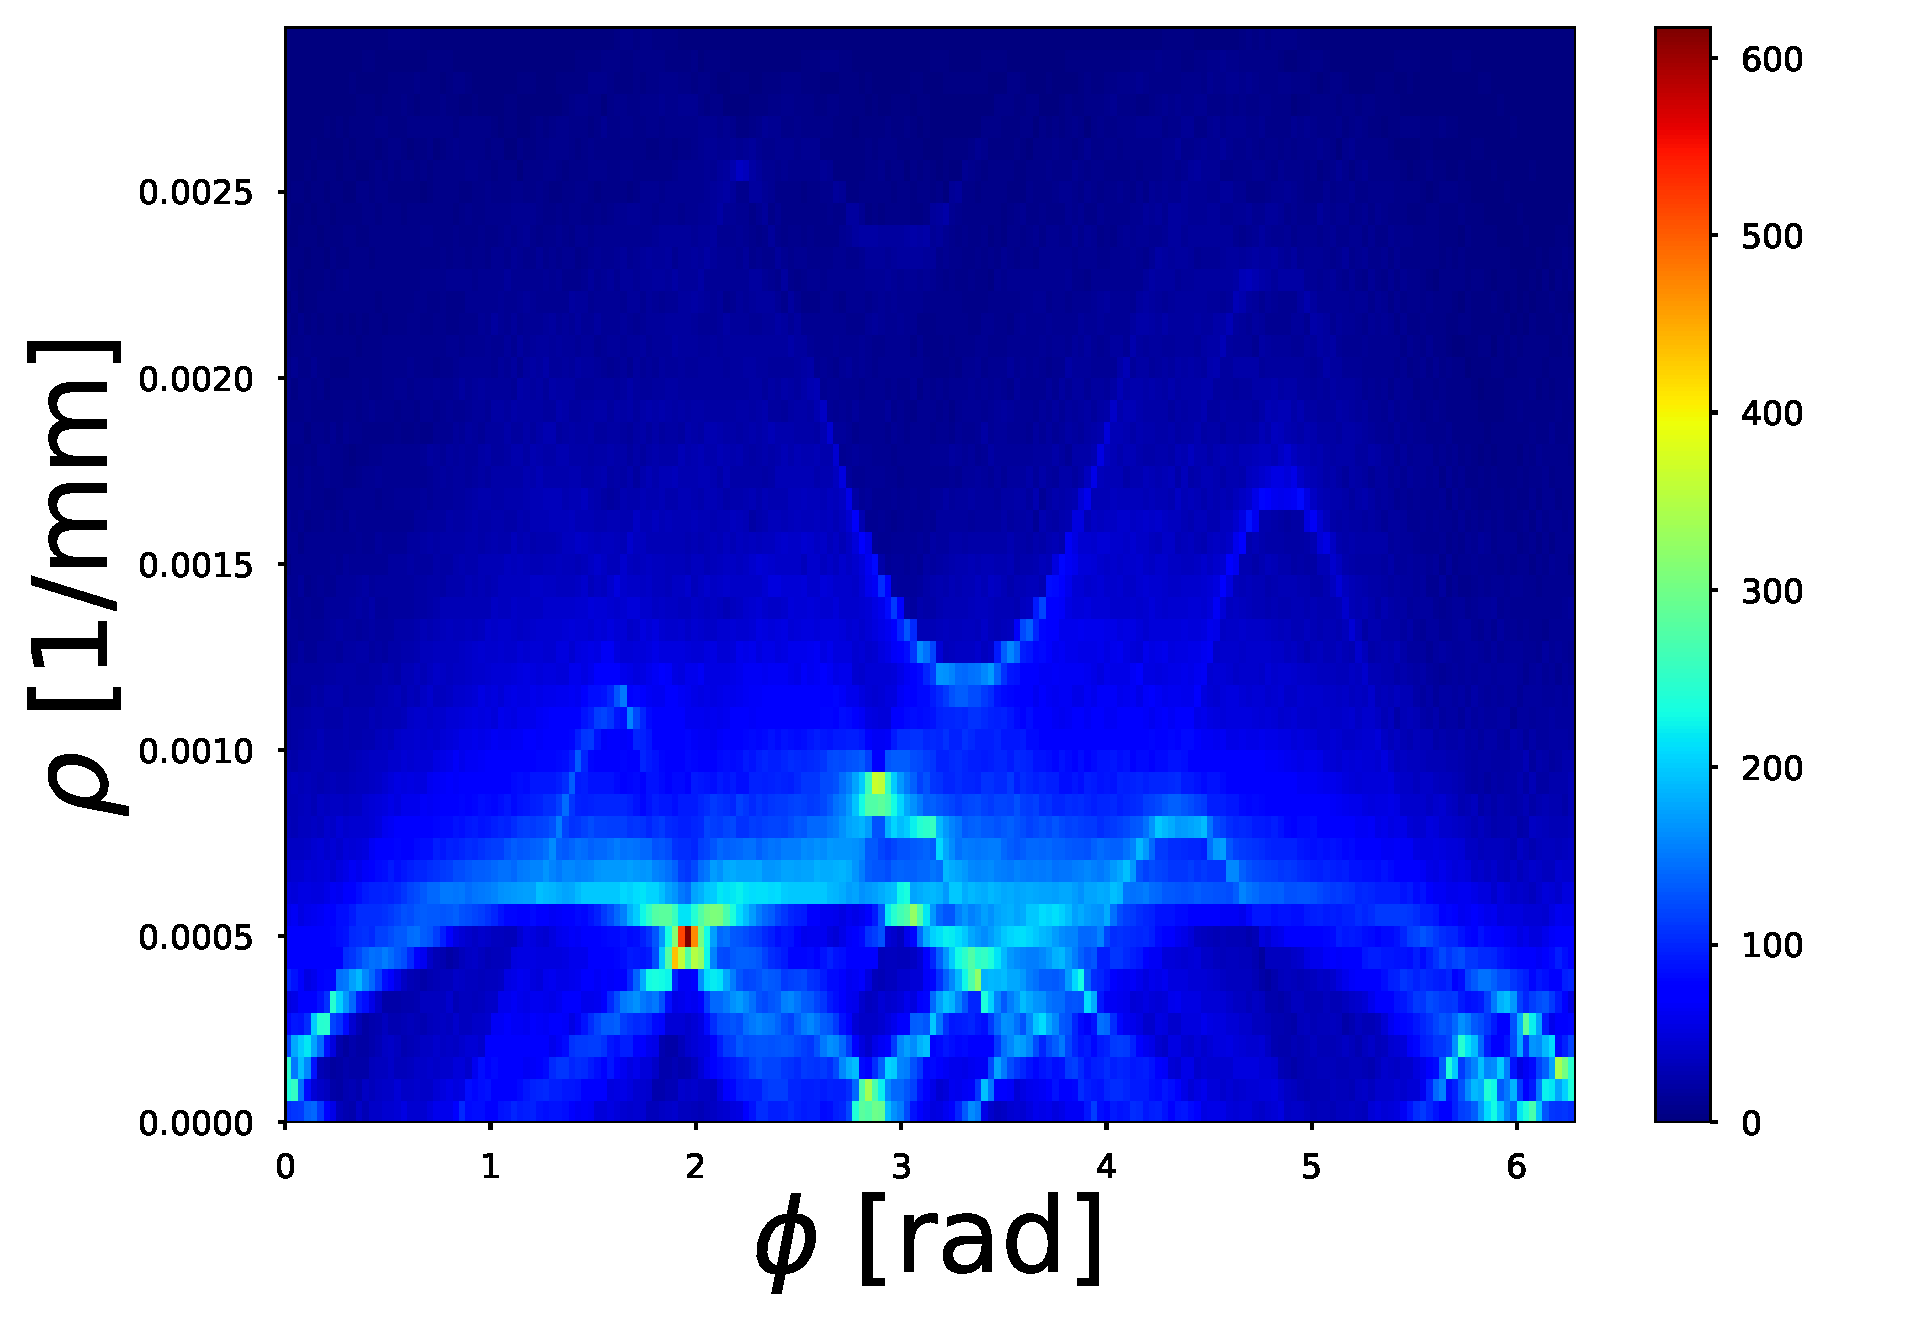
\includegraphics[width=0.8\textwidth]{figures/HT_Zdd.pdf}
	\label{HTZdd}
	\caption{The Hough transformation corresponding to the Z $\rightarrow$ d\={d} decay.}
\end{figure}
